% !TEX program = LuaLaTeX
% !TEX encoding = UTF-8 Unicode
% !TEX spellcheck = en_US

% --------------------------------------------------------------------------- %
% Poster template for Institute of Telematics.      						  %
% --------------------------------------------------------------------------- %
% Created with Brian Amberg's LaTeX Poster Template. Please refer to the     %
% attached README.md file for the details of how to compile.				      %
% --------------------------------------------------------------------------- %
% $LastChangedDate:: 2017-08-03 18:00:00 +0200 (V, 12 szept. 2017)          $ %
% $LastChangedRevision:: 129                                                $ %
% $LastChangedBy:: allner                                                   $ %
% $Id:: poster.tex 128 2011-09-11 08:57:12Z rlegendi                        $ %
% --------------------------------------------------------------------------- %

\documentclass[a0paper,portrait]{baposter}

\usepackage[utf8]{inputenc}
\usepackage{relsize}		% For \smaller
\usepackage{url}			% For \url
\usepackage{epstopdf}		% Included EPS files automatically converted to PDF to include with pdf latex
\usepackage{verbatimbox}
\usepackage{enumitem}
\usepackage{wrapfig}
\usepackage{natbib}
\usepackage{setspace}
\usepackage{uzlcolor}
\usepackage[english]{babel}
\usepackage{blindtext}
\usepackage{caption}
\usepackage{setspace}

%%% Myriad Pro Font - %%%%%%%%%%%%%%%%%%%%%%%%%%%%%%%%%%%%%%%%%%%%%%%%%%%%%%%%%
\usepackage{fontspec}
\defaultfontfeatures{Ligatures=TeX,Scale=MatchLowercase}
\setmonofont{Myriad Pro}
\setmainfont[
BoldFont={Myriad Pro}, 
ItalicFont={Myriad Pro},
BoldItalicFont={Myriad Pro}
]{Myriad Pro}
\setsansfont{Myriad Pro}


%%% Global Settings %%%%%%%%%%%%%%%%%%%%%%%%%%%%%%%%%%%%%%%%%%%%%%%%%%%%%%%%%%%
\graphicspath{{pix/}}	% Root directory of the pictures 
%\tracingstats=2			% Enabled LaTeX logging with conditionals
\tracinglostchars=2		% Enabled character loss logging

\newcommand{\localtextbulletone}{\textcolor{uzl_orange_2}{\raisebox{0.2ex}{\rule{1.2ex}{1.2ex}}}}
\renewcommand{\labelitemi}{\localtextbulletone}

%%%%%%%%%%%%%%%%%%%%%%%%%%%%%%%%%%%%%%%%%%%%%%%%%%%%%%%%%%%%%%%%%%%%%%%%%%%%%%%%
%%% Utility functions %%%%%%%%%%%%%%%%%%%%%%%%%%%%%%%%%%%%%%%%%%%%%%%%%%%%%%%%%%

%%% Save space in lists. Use this after the opening of the list %%%%%%%%%%%%%%%%
\newcommand{\compresslist}{
	\setlength{\itemsep}{1pt}
	\setlength{\parskip}{0pt}
	\setlength{\parsep}{0pt}
}

\renewcommand{\familydefault}{\sfdefault}


%%%%%%%%%%%%%%%%%%%%%%%%%%%%%%%%%%%%%%%%%%%%%%%%%%%%%%%%%%%%%%%%%%%%%%%%%%%%%%%
%%% Document Start %%%%%%%%%%%%%%%%%%%%%%%%%%%%%%%%%%%%%%%%%%%%%%%%%%%%%%%%%%%%
%%%%%%%%%%%%%%%%%%%%%%%%%%%%%%%%%%%%%%%%%%%%%%%%%%%%%%%%%%%%%%%%%%%%%%%%%%%%%%%
\begin{document}
% !TEX program = LuaLaTeX
% !TEX encoding = UTF-8 Unicode
% !TEX spellcheck = en_US

\begin{myverbbox}{\observewithouteid}
CLIENT                                       SERVER
  |                                            |
  |------------- CON [MID=1, T=0xAB, OBS] ---->|
  |                                            |
  |<----- ACK [MID=1, T=0xAB, OBS=1] ----------|
  |                                            |
  |                             (Server IP changes)
  |                                            |
  |<----- CON [MID=3, T=0xAB, OBS=2] ----------|
  |                                            |
  |---------------------- empty RST [MID=3] -->|
  |                                            |
\end{myverbbox}


\begin{myverbbox}{\observewitheid}
CLIENT                                       SERVER
  |                                            |
  |----- CON [MID=1, T=0xAB, OBS, EID1=0xCD]-->|
  |                                            |
  |<-- ACK [MID=1, T=0xAB, OBS=1, EID2=0xCD]---|
  |                                            |
  |                                    (Server IP changes)
  |                                            |
  |<-- CON [MID=3, T=0xAB, OBS=2, EID2=0xCD] --|
  |                                            |
  |---------------------- empty ACK [MID=3] -->|
  |                                            |
\end{myverbbox}


\begin{myverbbox}{\eidforclient}
   CLIENT                                       SERVER
      |                                            |
      |---------------- CON [MID=1, T=0xAB, OBS]-->|
      |                                            |
      |<-- ACK [MID=1, T=0xAB, OBS=1, EID1=0xEF ---|
      |                                            |
(Client IP changes)                                |
      |                                            |
      |---- CON [MID=5, T=0xAB, OBS, EID2=0xEF] -->|
      |                                            |
      |<-- ACK [MID=5, T=0xAB] --------------------|
      |                                            |
\end{myverbbox}


\begin{myverbbox}{\server}
   CLIENT                                       SERVER
    | \colorbox{white}{\ }                                          |
    |----- CON [MID=1, T=0xAB, OBS, \colorbox{yellow}{\textbf{EID1=0xCD}}]-->|
    | \colorbox{white}{\ }                                          |
    |<-- ACK [MID=1, T=0xAB, OBS=1, \colorbox{yellow}{\textbf{EID2=0xCD}}]---|
    | \colorbox{white}{\ }                                          |
    | \colorbox{white}{\ }                                (Server IP changes)
    | \colorbox{white}{\ }                                          |
    |<-- CON [MID=5, T=0xAB, OBS=2, \colorbox{yellow}{\textbf{EID2=0xCD]}} --|
    | \colorbox{white}{\ }                                          |
    |---------------------- empty ACK\colorbox{white}{\ }[MID=5] -->|
    | \colorbox{white}{\ }                                          |
\end{myverbbox}


\typeout{Poster rendering started}

%%% Setting Background Image %%%%%%%%%%%%%%%%%%%%%%%%%%%%%%%%%%%%%%%%%%%%%%%%%%
\background{
% 	\begin{tikzpicture}[remember picture,overlay]%
% 	\draw (current page.north west)+(-2em,2em) node[anchor=north west]
% 	{\includegraphics[height=1.1\textheight]{background}}
% 	\end{tikzpicture}
}

%%% General Poster Settings %%%%%%%%%%%%%%%%%%%%%%%%%%%%%%%%%%%%%%%%%%%%%%%%%%%
%%%%%% Eye Catcher, Title, Authors and University Images %%%%%%%%%%%%%%%%%%%%%%
\begin{poster}{
	grid=false,
	% Option is left on true though the eyecatcher is not used. The reason is
	% that we have a bit nicer looking title and author formatting in the headercol
	% this way
	eyecatcher=false, 
	borderColor=uzl_oceangreen_80,
	headerColorOne=uzl_oceangreen_80,
	headerColorTwo=uzl_oceangreen_80,
	headerFontColor=white,
	% Only simple background color is used, no shading, so boxColorTwo isn't necessary
	boxColorOne=white,
	% rectangle small-rounded rounded right rounded left rounded
	headershape=rectangle,
	headerfont=\large\bf,
	% none bars coils triangles rectangle rounded faded
	textborder=roundedsmall,
	background=plain,
	bgColorOne=white,
	% none closed open
	headerborder=open,
	% plain shade-lr shade-tb none
	boxshade=plain,
	%Number of columns (default 4 in landscape and 3 in portrait format) (maximum is 6)
	%colspacing=length
	columns=5,
	linewidth=1pt,
	% plain shade-lr shade-tb shade-tb-inverse
	headershade=plain
}
%%% Eye Cacther %%%%%%%%%%%%%%%%%%%%%%%%%%%%%%%%%%%%%%%%%%%%%%%%%%%%%%%%%%%%%%%
{
%  \includegraphics[height=5em]{qrcode}
%  \hspace{0.7cm}
}
%%% Title %%%%%%%%%%%%%%%%%%%%%%%%%%%%%%%%%%%%%%%%%%%%%%%%%%%%%%%%%%%%%%%%%%%%%
{
	\vspace{0.3cm}
	\begin{minipage}{\linewidth}
	  \setstretch{0.7}
	  \textcolor{uzl_oceangreen_80}{\textbf{Flexible API for IoT Services with Named Data}} \\
	  \textcolor{uzl_oceangreen_80}{\textbf{Networking}}
	\end{minipage}
	\vspace{0.3cm}
}
%%% Subtitle %%%%%%%%%%%%%%%%%%%%%%%%%%%%%%%%%%%%%%%%%%%%%%%%%%%%%%%%%%%%%%%%%%%
{
  \textcolor{uzl_orange_2}{\textsf{}}
}
%%% Logo %%%%%%%%%%%%%%%%%%%%%%%%%%%%%%%%%%%%%%%%%%%%%%%%%%%%%%%%%%%%%%%%%%%%%%
{
  \hspace{1cm}
  
\includegraphics[height=8em]{Logo_Inst_Telematik_orig}
}

%%% Header %%%%%%%%%%%%%%%%%%%%%%%%%%%%%%%%%%%%%%%%%%%%%%%%%%%%%%%%%%%%%%%%%%%%%
\headerbox{}{name=headtext, column=0, span=5, textborder=none, headerborder=none, boxheaderheight=0pt, boxColorOne=uzl_oceangreen_80}{
  \vspace{0.10cm}
    \textcolor{white}{\textsf{\large{Christopher Horn  \hfill - \hfill Universitaet zu Luebeck \hfill - \hfill Institut fuer Telematik \hfill - \hfill Email: christopher.horn@student.uni-luebeck.de}}}
  \vspace{0.10cm}
}


%%% I. Abschnitt %%%%%%%%%%%%%%%%%%%%%%%%%%%%%%%%%%%%%%%%%%%%%%%%%%%%%%%%%%%%%%%%%%%%%
\headerbox{Introduction}{name=abschnitt1, column=0, span=3, row=0, below=headtext}{
	\vspace{0.5em}
	\begin{itemize}[leftmargin=5.5mm, rightmargin=5.5mm]
        \item The Internet of Things (IoT) significantly enhances our daily activities through a myriad of applications and services provided by interconnected devices.
		\item IoT devices collect environmental data and monitor various events when connected to the internet, necessitating efficient integration methods with IoT applications.
		\item Named Data Networking (NDN) emerges as a potent solution to facilitate device and service integration, aligning with the Information-Centric Networking (ICN) paradigm for future network advancements \cite{ahlgren2012survey} \cite{zhang2010named}.
		\item This paper introduces a novel API tailored for IoT services in an NDN environment, refining the communication between IoT devices and services.
	\end{itemize}
	\vspace{0.5em}
}

%%% II. Abschnitt %%%%%%%%%%%%%%%%%%%%%%%%%%%%%%%%%%%%%%%%%%%%%%%%%%%%%%%%%%%%%%%%%%%%%
\headerbox{\textsf{API for IoT Services}}{name=abschnitt2,column=0, span=3, below=abschnitt1}{
	\vspace{0.5em}
	\begin{itemize}[leftmargin=5.5mm, rightmargin=5.5mm]
		\item IoT services provide crucial data from sensors and network environments, aiding decision-making processes \cite{hail2015iot}.
        \item The proposed API aims to streamline the incorporation of services within the IoT-NDN framework, as depicted in Figure 1.
		\item Services, acting as modular system components, are essential for delivering information from device sensors and network environments, aiding in decision-making across various sectors.
		\item The API's design ensures adaptability for any service within the IoT-NDN system, fostering seamless information sharing and retrieval.
		\item A service-oriented integration is emphasized, catering to the constraints of IoT devices and promoting real-time protocols and smart technology movements.
	\end{itemize}
	\vspace{0.5em}
}
 

%%% III. Abschnitt %%%%%%%%%%%%%%%%%%%%%%%%%%%%%%%%%%%%%%%%%%%%%%%%%%%%%%%%%%%%%%%%%%%%%
\headerbox{\textsf{Implementation}}{name=abschnitt3, column=0, span=3, below=abschnitt2}{


\vspace{0.5em}
	Naming Concept for IoT Services:
	\begin{itemize}[leftmargin=5.5mm, rightmargin=5.5mm]
        \item NDN offers flexible data requests with hierarchically structured, human-friendly names \cite{amadeo2014named}.
		\item A structured naming concept is introduced for IoT services, which includes COMMAND, COMMAND ID, and COMMAND PARAMETER as illustrated in Figure 2.
		\item This naming structure enables the transmission of various information types and allows for the efficient retrieval of general service information.
	\end{itemize}

    Deployment of IoT Services:
	\begin{itemize}[leftmargin=5.5mm, rightmargin=5.5mm]
        \item IoT services, small software units, monitor events and provide specific knowledge, enhancing decision-making efficiency.
		\item API architecture and service registration process demonstrated in Figure 3.
		\item Service integration involves the exchange of Interest/Data packets between IoT-Services and IoT-NDN layers.
		\item Example service registration for network time synchronization detailed, showcasing API's flexibility and integration benefits  \cite{zhang2010named}.
	\end{itemize}
		\vspace{0.5em}
}

%%% IV. Abschnitt %%%%%%%%%%%%%%%%%%%%%%%%%%%%%%%%%%%%%%%%%%%%%%%%%%%%%%%%%%%%%%%%%%%%%
\headerbox{\textsf{Conclusion}}{name=abschnitt4, column=0, span=3, below=abschnitt3, above=bottom}{
	
	\vspace{0.5em}
	\begin{itemize}[leftmargin=5.5mm, rightmargin=5.5mm]
        \item Recaps the innovative approach of the flexible API in the context of IoT and NDN.
        \item Highlights the API's successful implementation and its potential to transform IoT service integration.
        \item Example of network time synchronization service highlights API's flexibility and integration benefits.
        \item Future work includes testing API with more services and further development for enhanced usability. 
    \end{itemize}
	\vspace{0.5em}
}


%%% Bild 1 %%%%%%%%%%%%%%%%%%%%%%%%%%%%%%%%%%%%%%%%%%%%%%%%%%%%%%%%%%%%%%%%%%%%%
\headerbox{\textsf{Figure 1}}{name=bild1, column=3, span=2, below=headtext}{
	\vspace{0.5cm}
	\begin{center}
		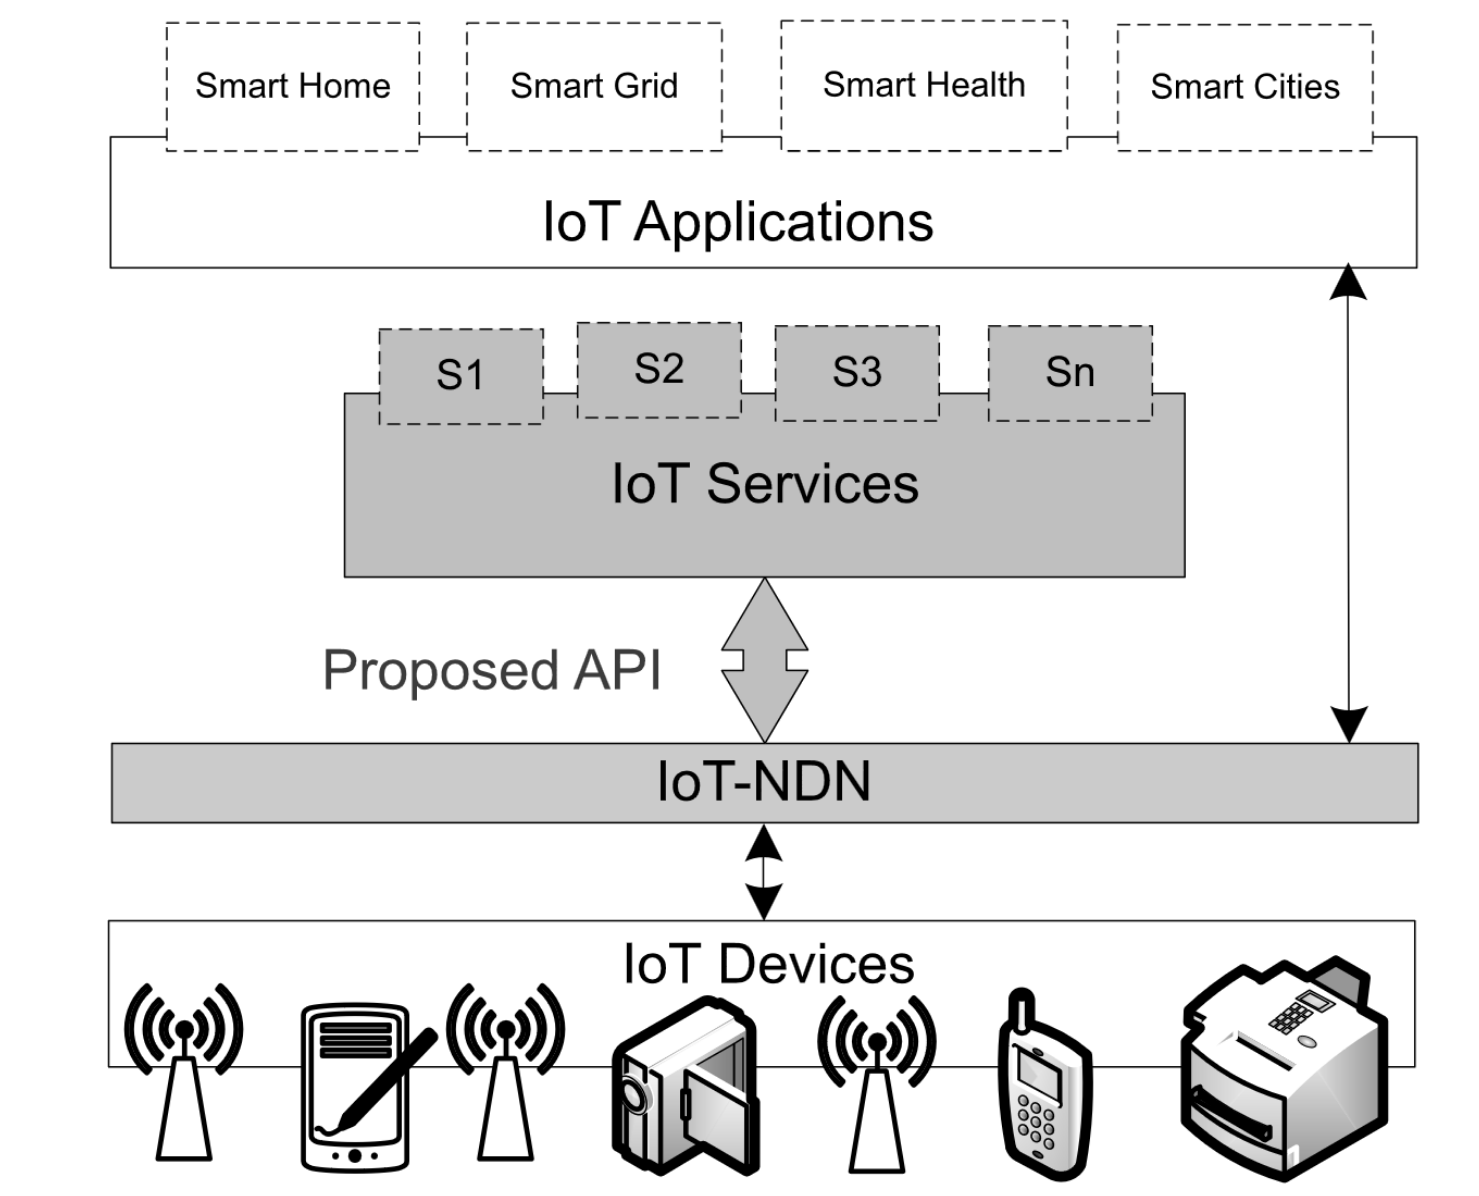
\includegraphics[width=0.7\textwidth]{figure_1_poster.png}
		% \captionof{figure}{The proposed API for IoT-Services using IoT-NDN}
		\label{fig:figure_1}
	\end{center}
	\vspace{0.5cm}
}


%%% Bild 2 %%%%%%%%%%%%%%%%%%%%%%%%%%%%%%%%%%%%%%%%%%%%%%%%%%%%%%%%%%%%%%%%%%%%%
\headerbox{\textsf{Figure 2}}{name=bild2,column=3, span=2, below=bild1}{
	\vspace{0.5cm}
	\begin{center}
			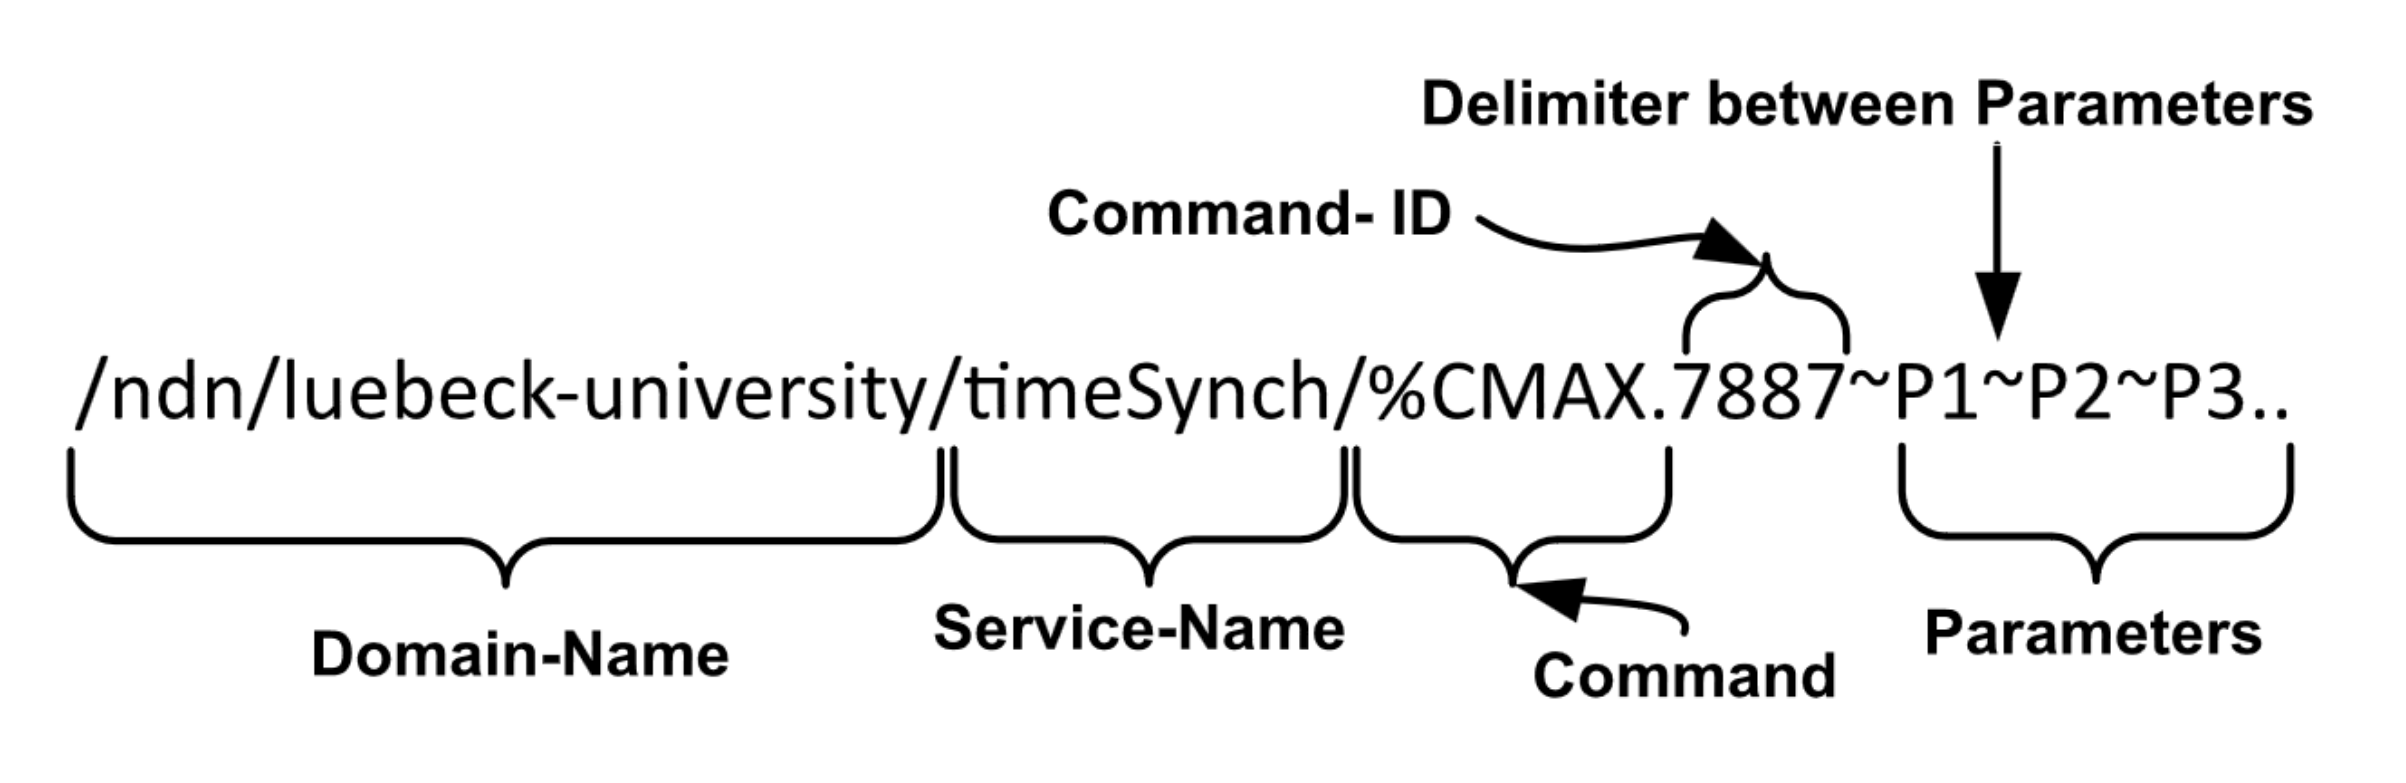
\includegraphics[width=0.9\textwidth]{figure_2_poster.png}
			% \captionof{figure}{Name Structure for IoT services including commands and their parameters}
			\label{fig:figure_2}
	\end{center}
	\vspace{0.5cm}
}


%%% Bild 3 %%%%%%%%%%%%%%%%%%%%%%%%%%%%%%%%%%%%%%%%%%%%%%%%%%%%%%%%%%%%%%%%%%%%%
\headerbox{\textsf{Figure 3}}{name=bild3, column=3, span=2, below=bild2}{
	\vspace{0.5cm}
	\begin{center}
			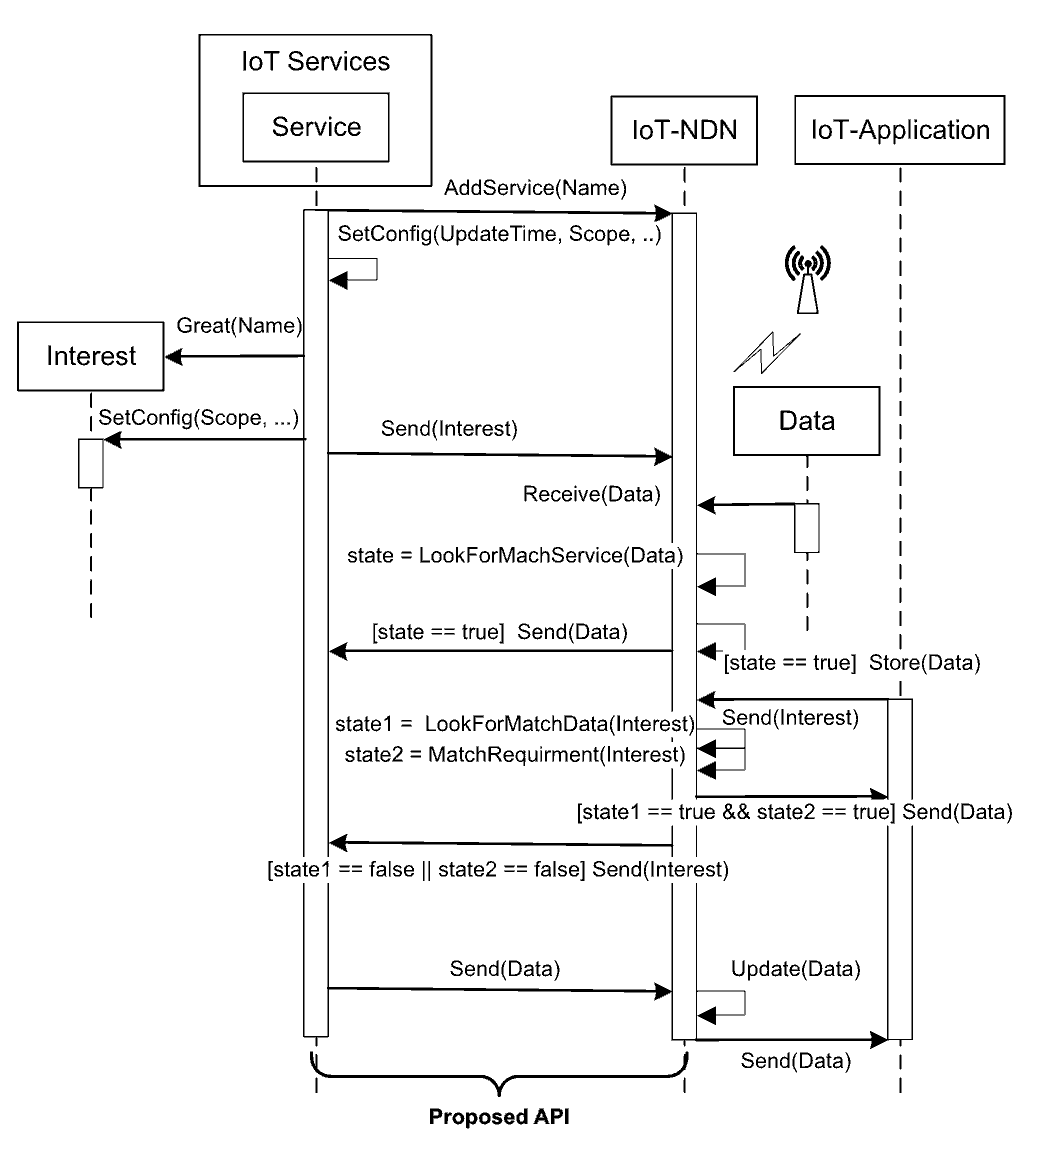
\includegraphics[width=0.9\textwidth]{figure_3_poster.png}
			% \captionof{figure}{Example of Service Integration and Exchange of Interest and Data Packets in IoT-NDN with the proposed API}
			\label{fig:figure_3}
	\end{center}
}


%%% References %%%%%%%%%%%%%%%%%%%%%%%%%%%%%%%%%%%%%%%%%%%%%%%%%%%%%%%%%%%%%%%%%%%%%
\headerbox{\textsf{References}}{name=references, column=3, span=2, above=bottom, below=bild3}{
  \begin{small}
  \renewcommand{\refname}{\vspace{-0.8em}}
  \setlength{\parskip}{0cm}
  \setlength{\bibsep}{0cm}
  \bibliographystyle{unsrt}
  \bibliography{references}
  \end{small}
}
\end{poster}
\end{document}
